\chapter{Вимірювання імпедансу за допомогою HP4192a} 
\label{chap:first}

У цій частині ми вчились приборкувати \sout{дракона} імпедансометр HP4192a. У нас було 3 завдання: дослідити залежність імпедансу від частоти для резистора, конденсатора та котушки.

\section{Вимірювання активного та реактивного опору резистора}

Отримана експеримантальним шляхом залежність активного та реактивного опору резистора від частоти не викликає сумнівів. Справді, активний опір не залежав істотно від частоти, та був приблизно рівним $95.4 \Omega$ упродовж всього експерименту. На рахунок реактивного опору - при високих частотах опір явно росте, що викликано індуктивними властивостями дротів, використаних у цьому резисторі. При малих частотах реактивний опір також росте, однак це вже викликано тим, що наш резистор в деякому сенсі працює як конденсатор.

\begin{figure}[h]
    \begin{minipage}[h]{0.47\linewidth}
        \center{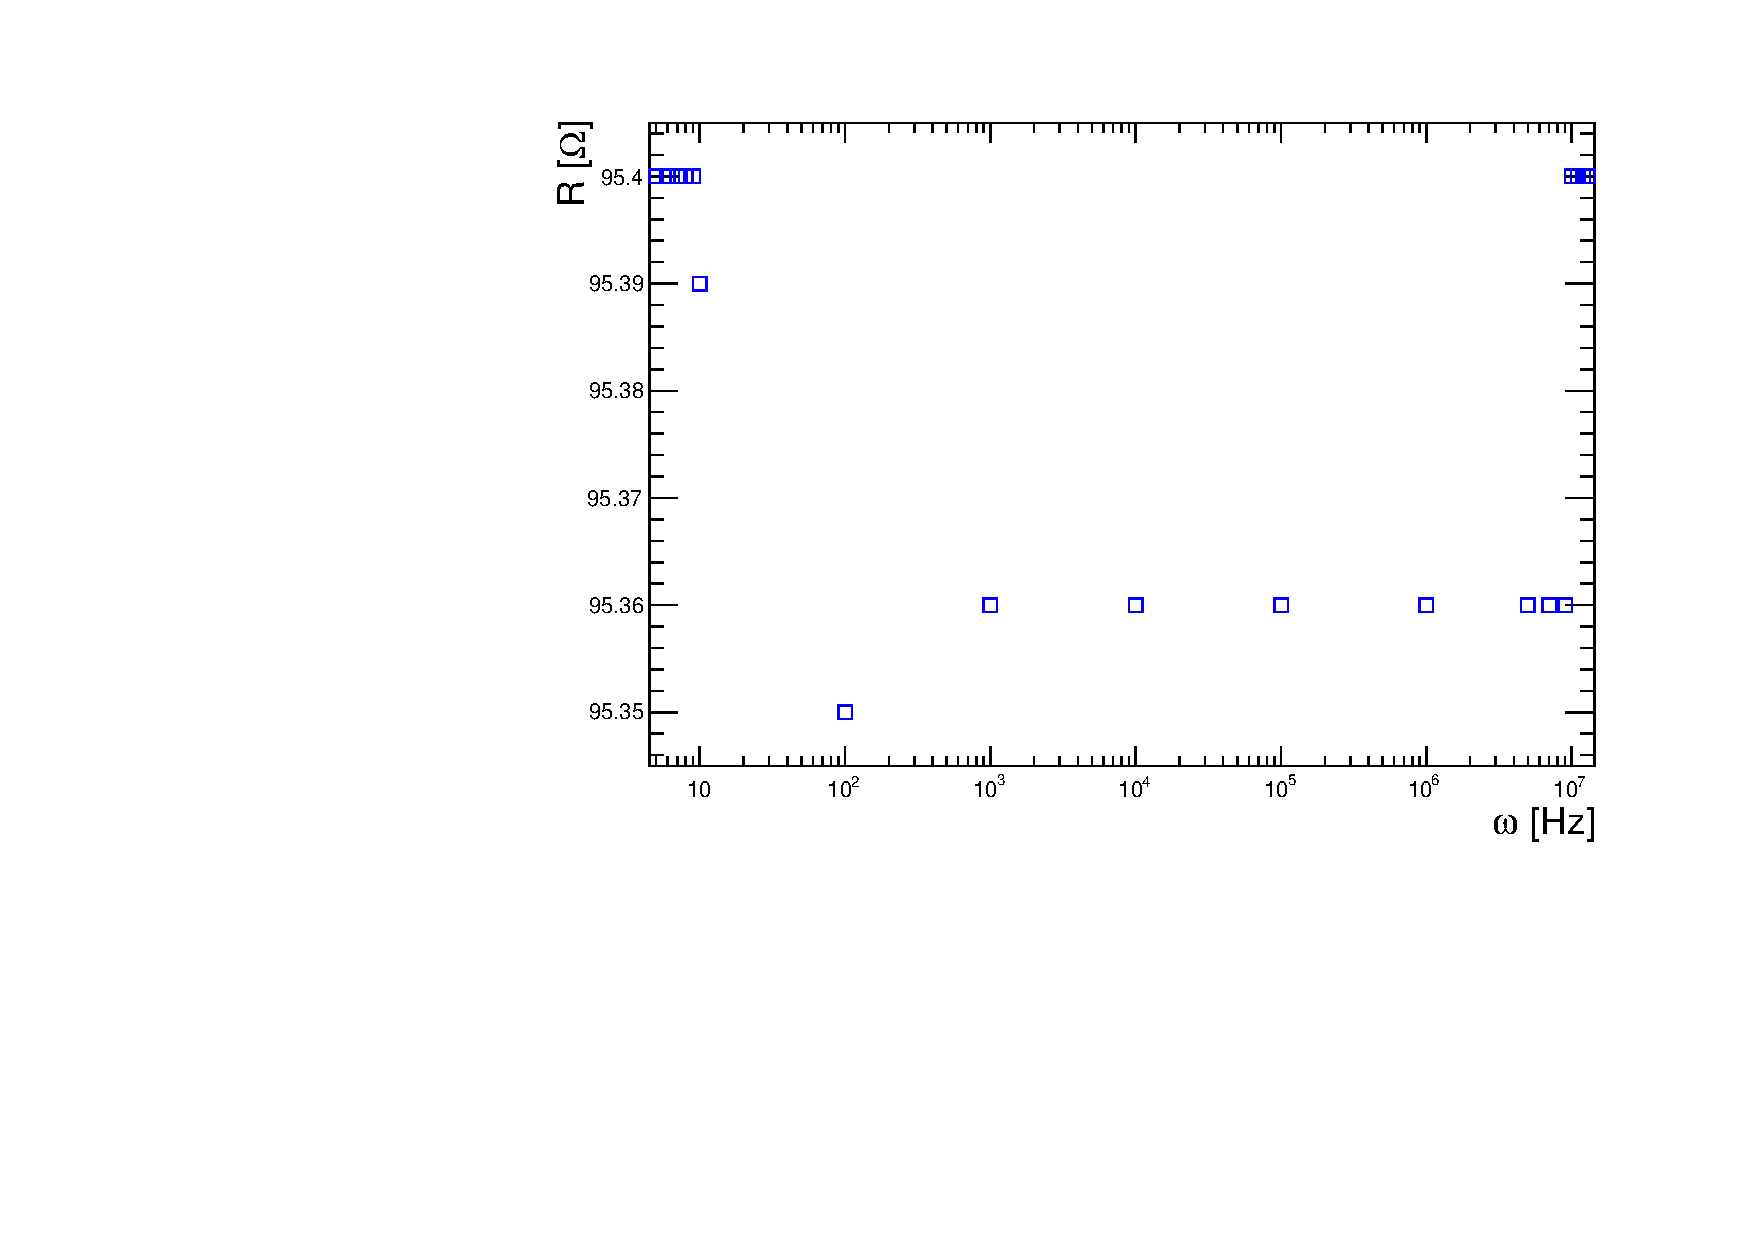
\includegraphics[width=1\linewidth]{pdf/c1_RR.pdf}} \\
    \end{minipage}
    \hfill
    \begin{minipage}[h]{0.47\linewidth}
        \center{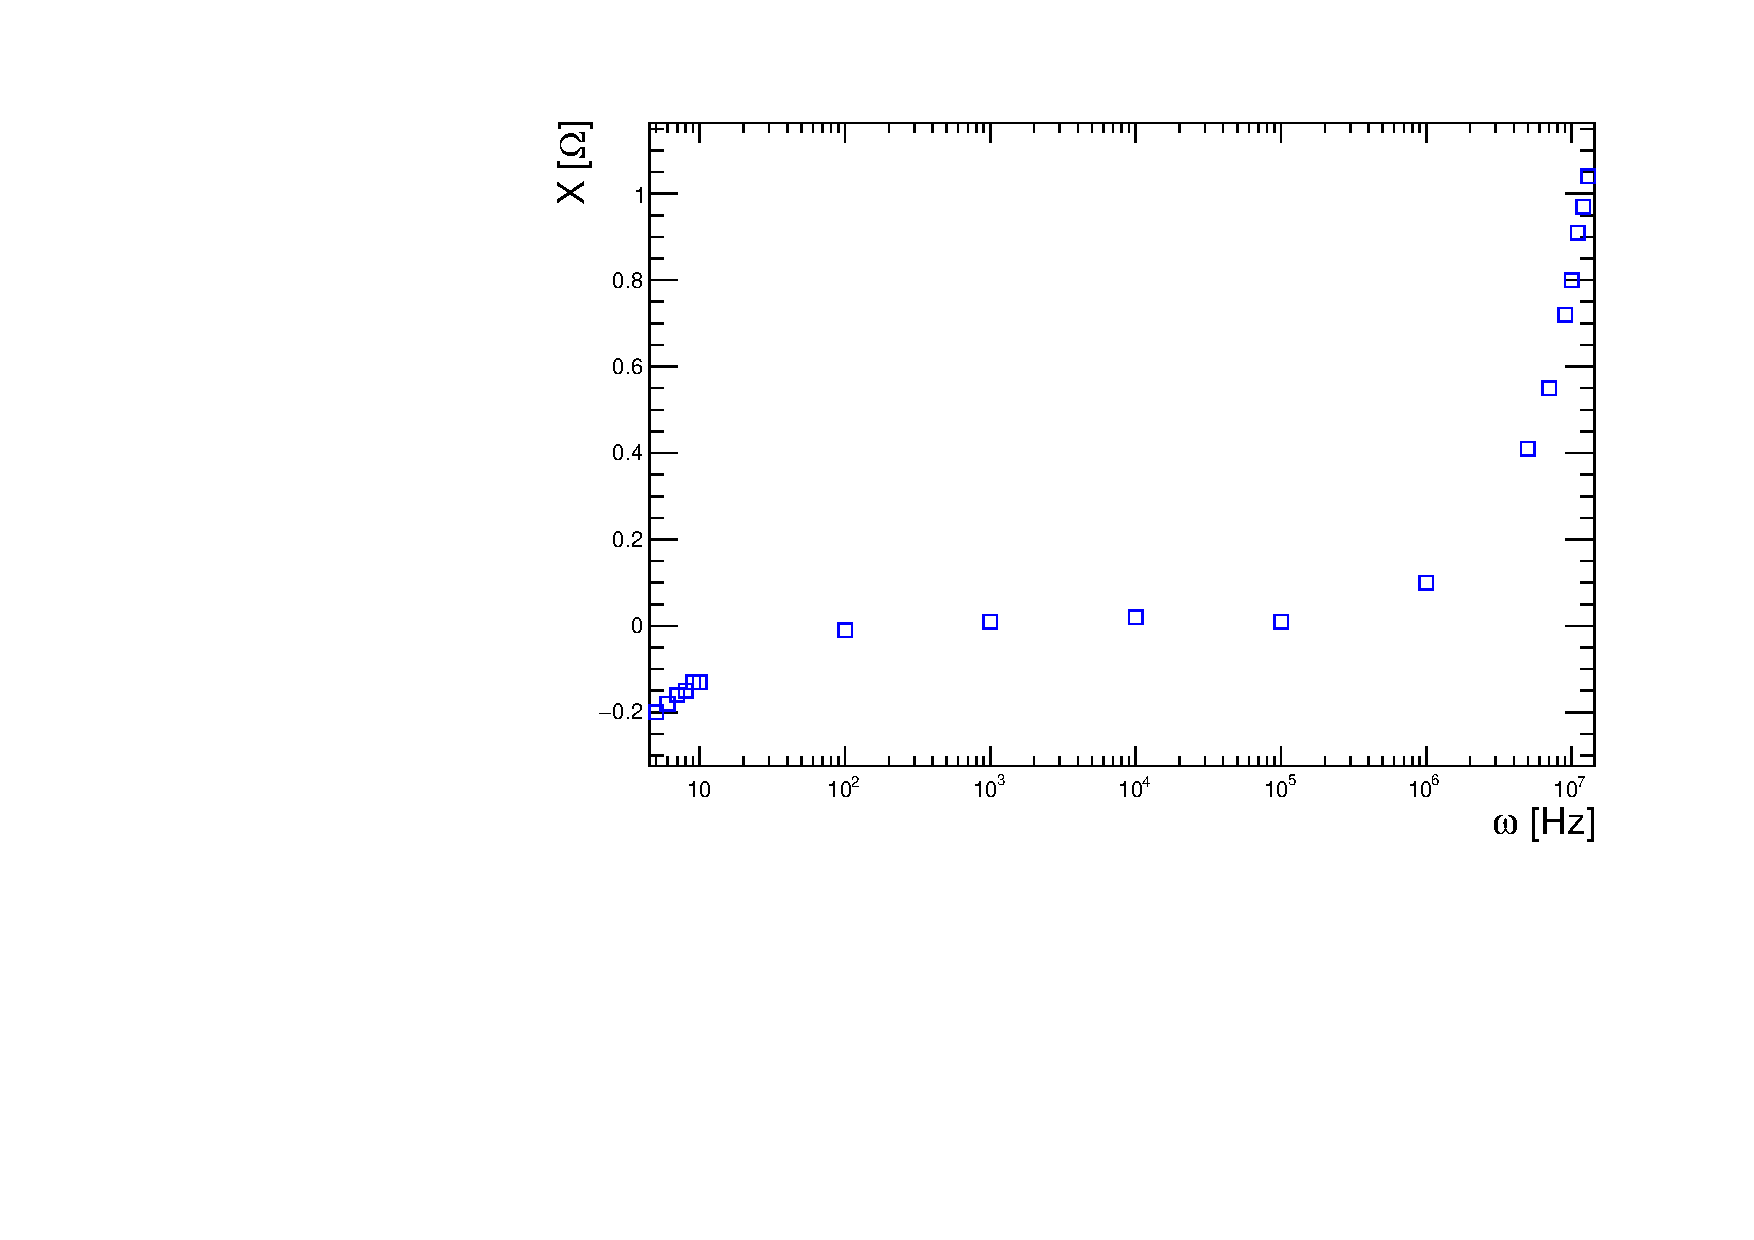
\includegraphics[width=1\linewidth]{pdf/c1_RX.pdf}}\\
    \end{minipage}
    \caption{Залежність активного та реактивного опору резистора від частоти}
    \label{fig:part21}
\end{figure}


\section{Вимірювання активного та реактивного опору конденсатора}

Отримана експеримантальним шляхом залежність активного та реактивного опору котушки від частоти виявилась досить цікавою. Справді, активний опір досить швидко обвалюється, що природньо, однак при $\omega \approx 10^7 Hz$ має досить дивний пік, що можливо пов'язано із властивостями діеелектрика всередині. Реактивний опір також швидко падає, маючи мінімум при $\omega \approx 10^5 Hz$, та після цього починає рости.

\begin{figure}[h]
    \begin{minipage}[h]{0.47\linewidth}
        \center{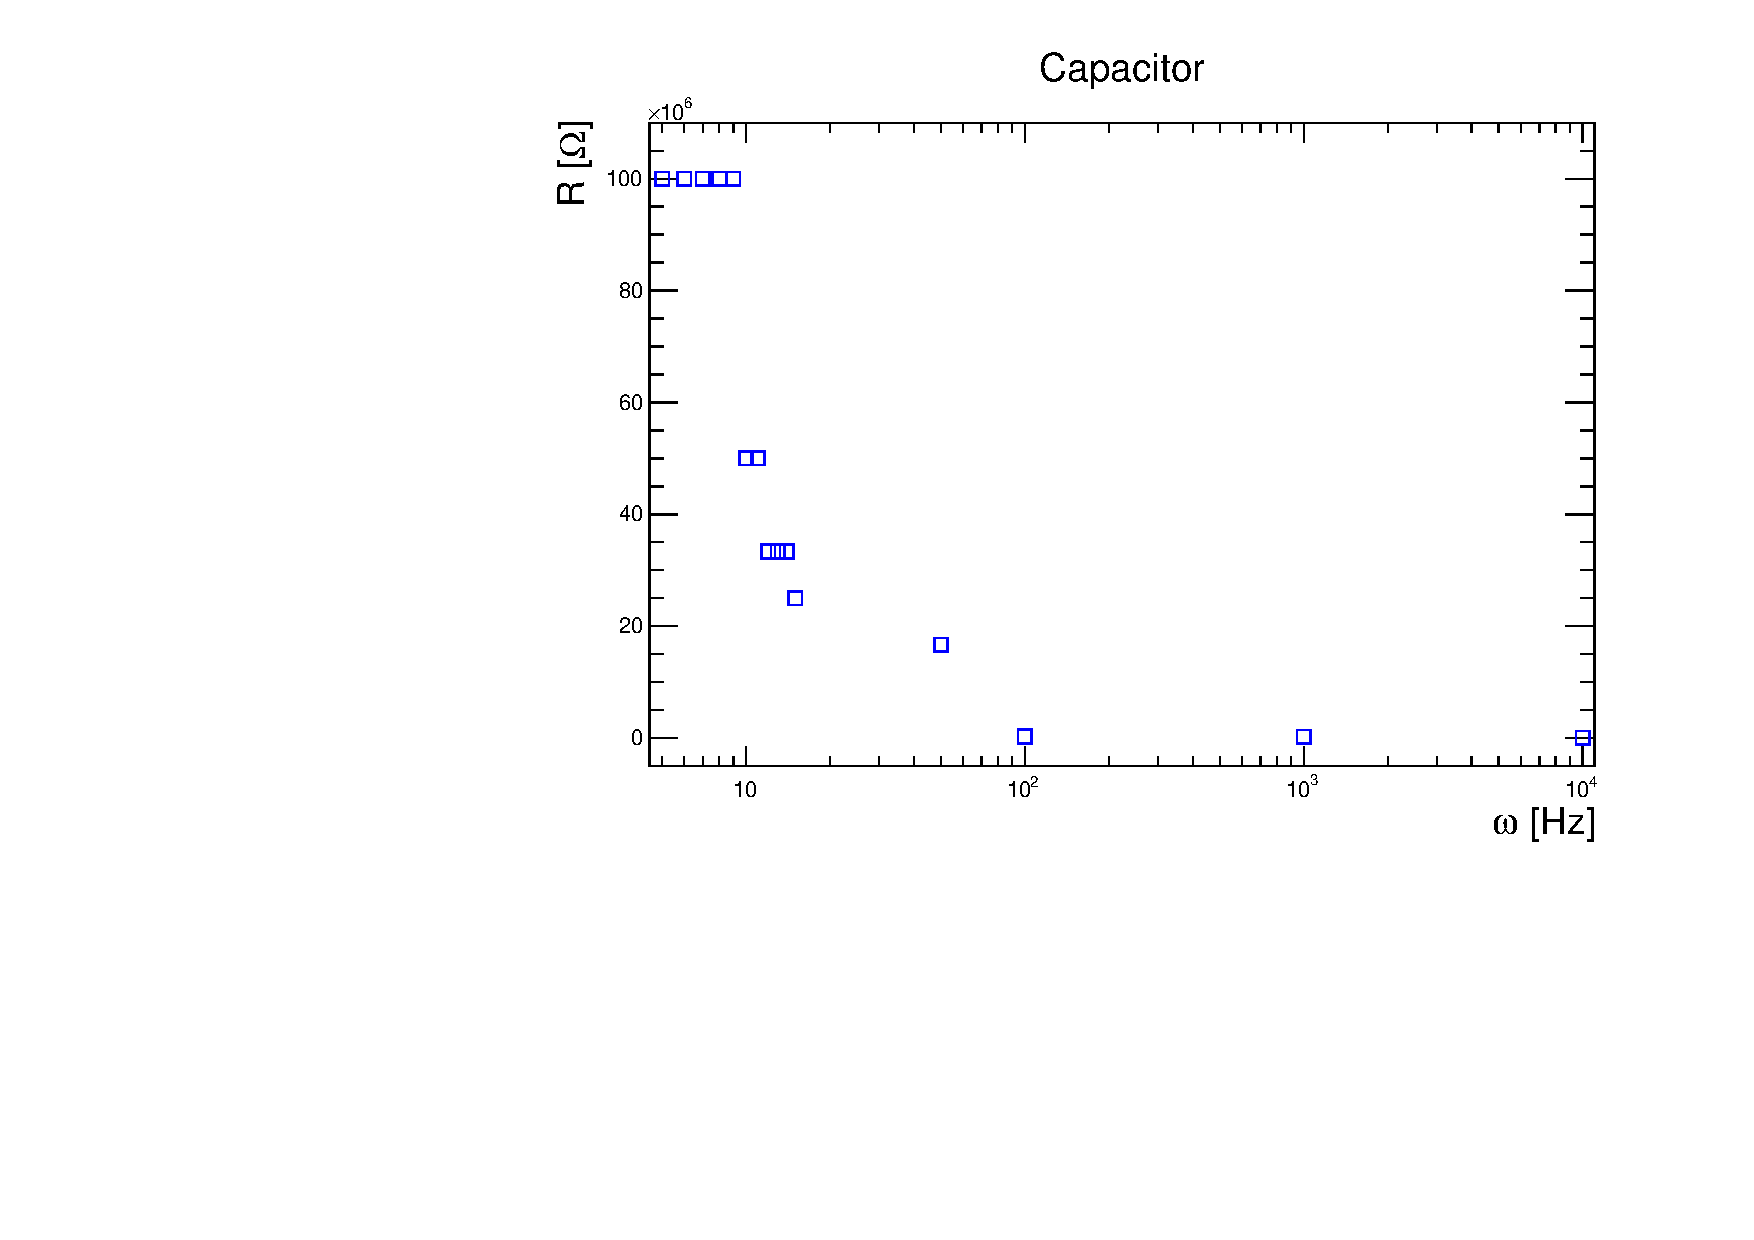
\includegraphics[width=1\linewidth]{pdf/c1_CR.pdf}} \\
    \end{minipage}
    \hfill
    \begin{minipage}[h]{0.47\linewidth}
        \center{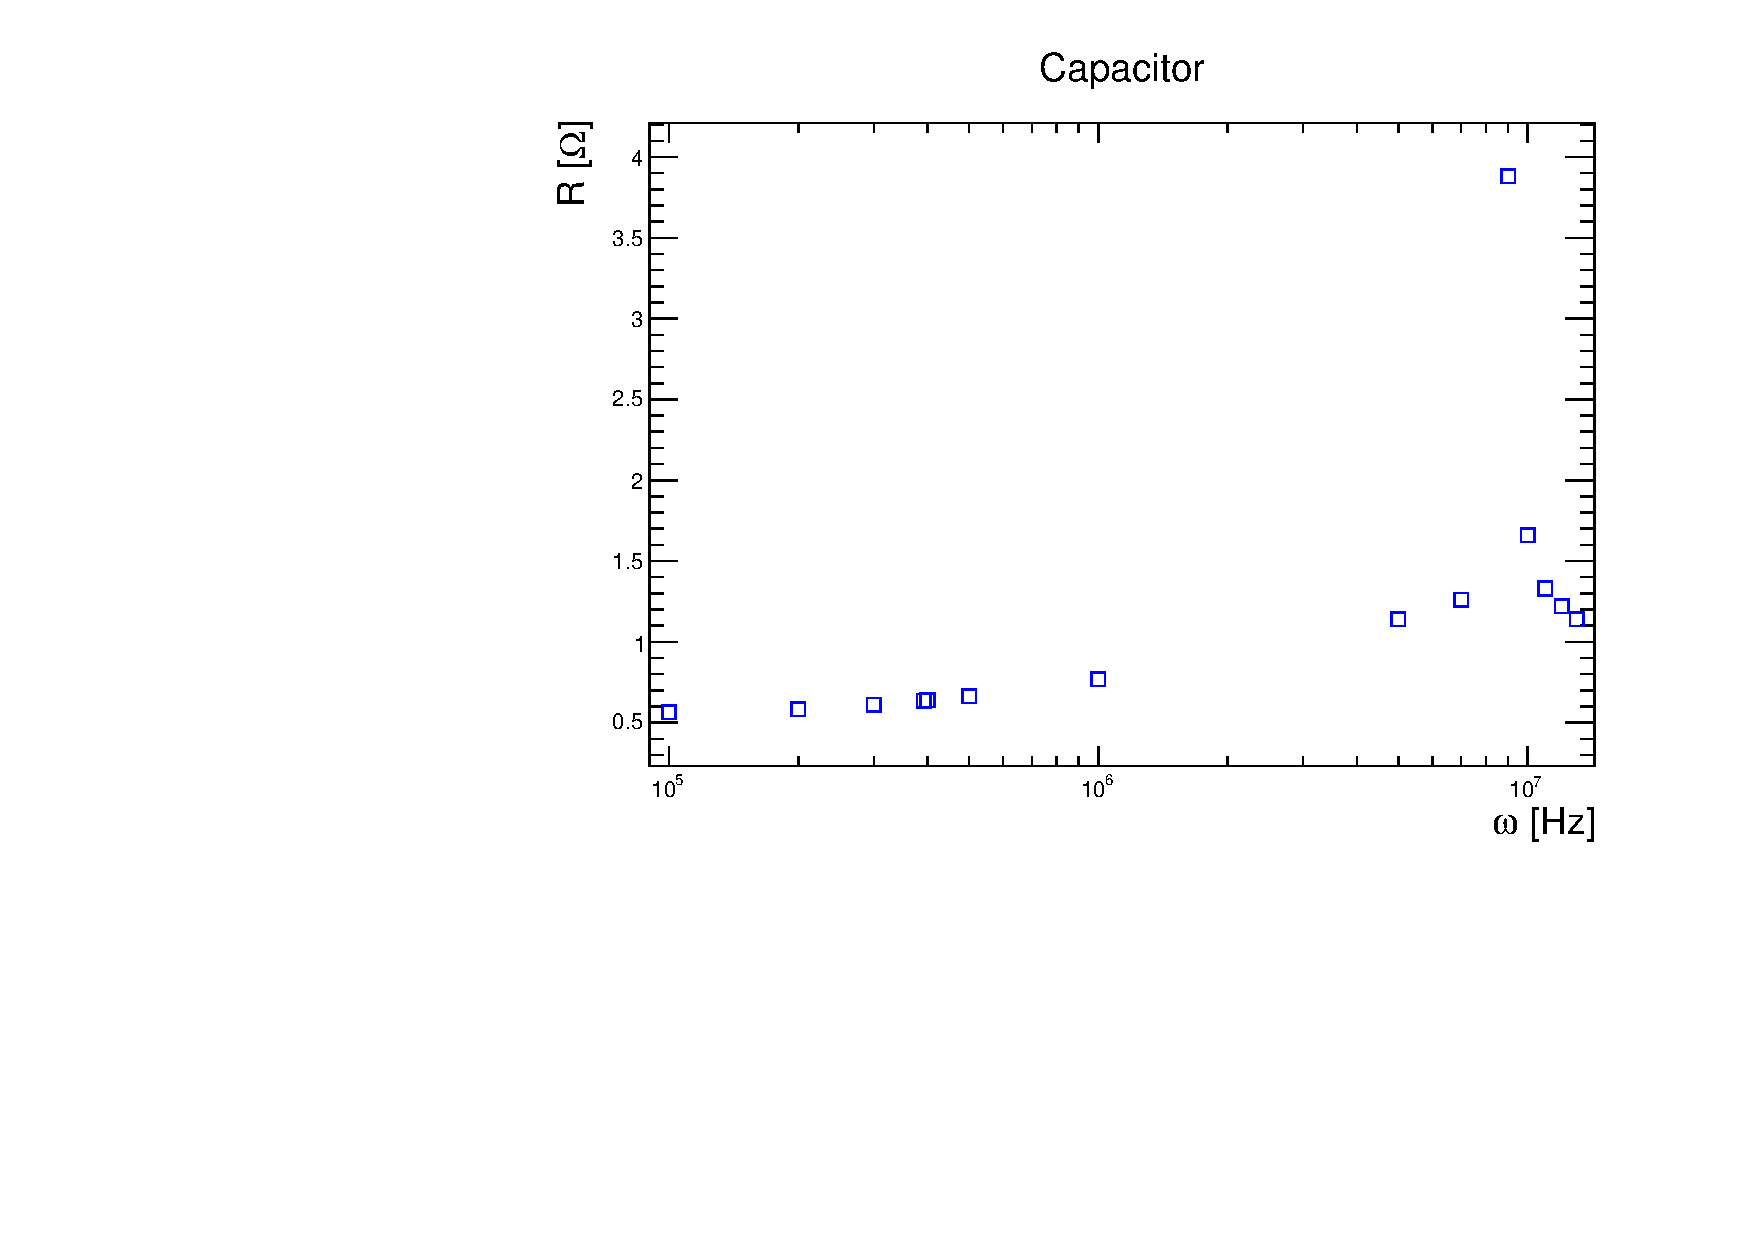
\includegraphics[width=1\linewidth]{pdf/c1_CR2.pdf}}\\
    \end{minipage}
    \vfill
    \begin{minipage}[h]{0.47\linewidth}
        \center{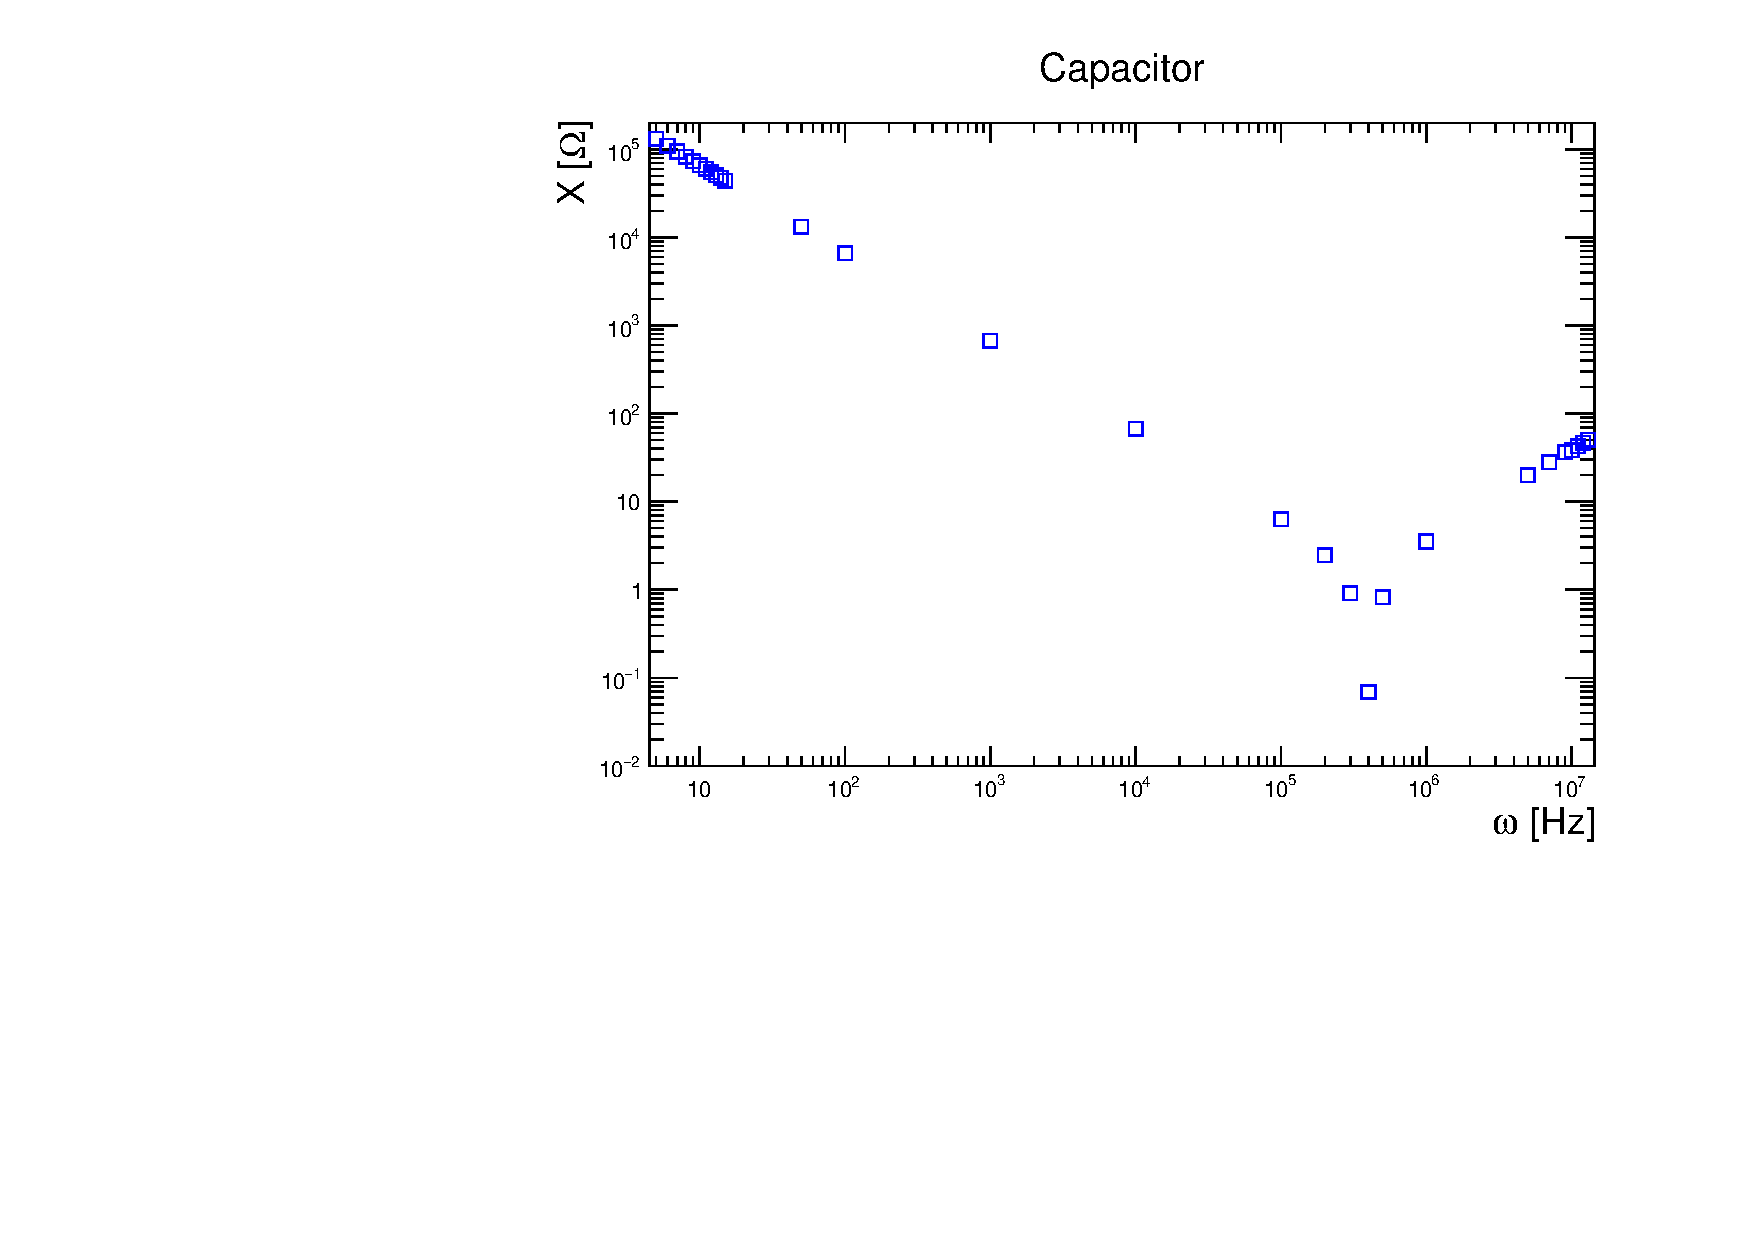
\includegraphics[width=1\linewidth]{pdf/c1_CX.pdf}}\\
    \end{minipage}
    \caption{Залежність активного та реактивного опору конденсатора від частоти}
    \label{fig:part22}
\end{figure}

\section{Вимірювання активного та реактивного опору котушки}

Отримана експеримантальним шляхом залежність активного та реактивного опору котушки від частоти викликає бажання у автора спитати викладача про доцільність даного експерименту. Справді, поведінка активного опіру може бути охарактеризована прекрасною фразою брєд сивої кобили. Хоча пік реактивного опору в районі $\omega \approx 10^6 Hz$ виглядає досить цікавим.

\begin{figure}[h]
    \begin{minipage}[h]{0.47\linewidth}
        \center{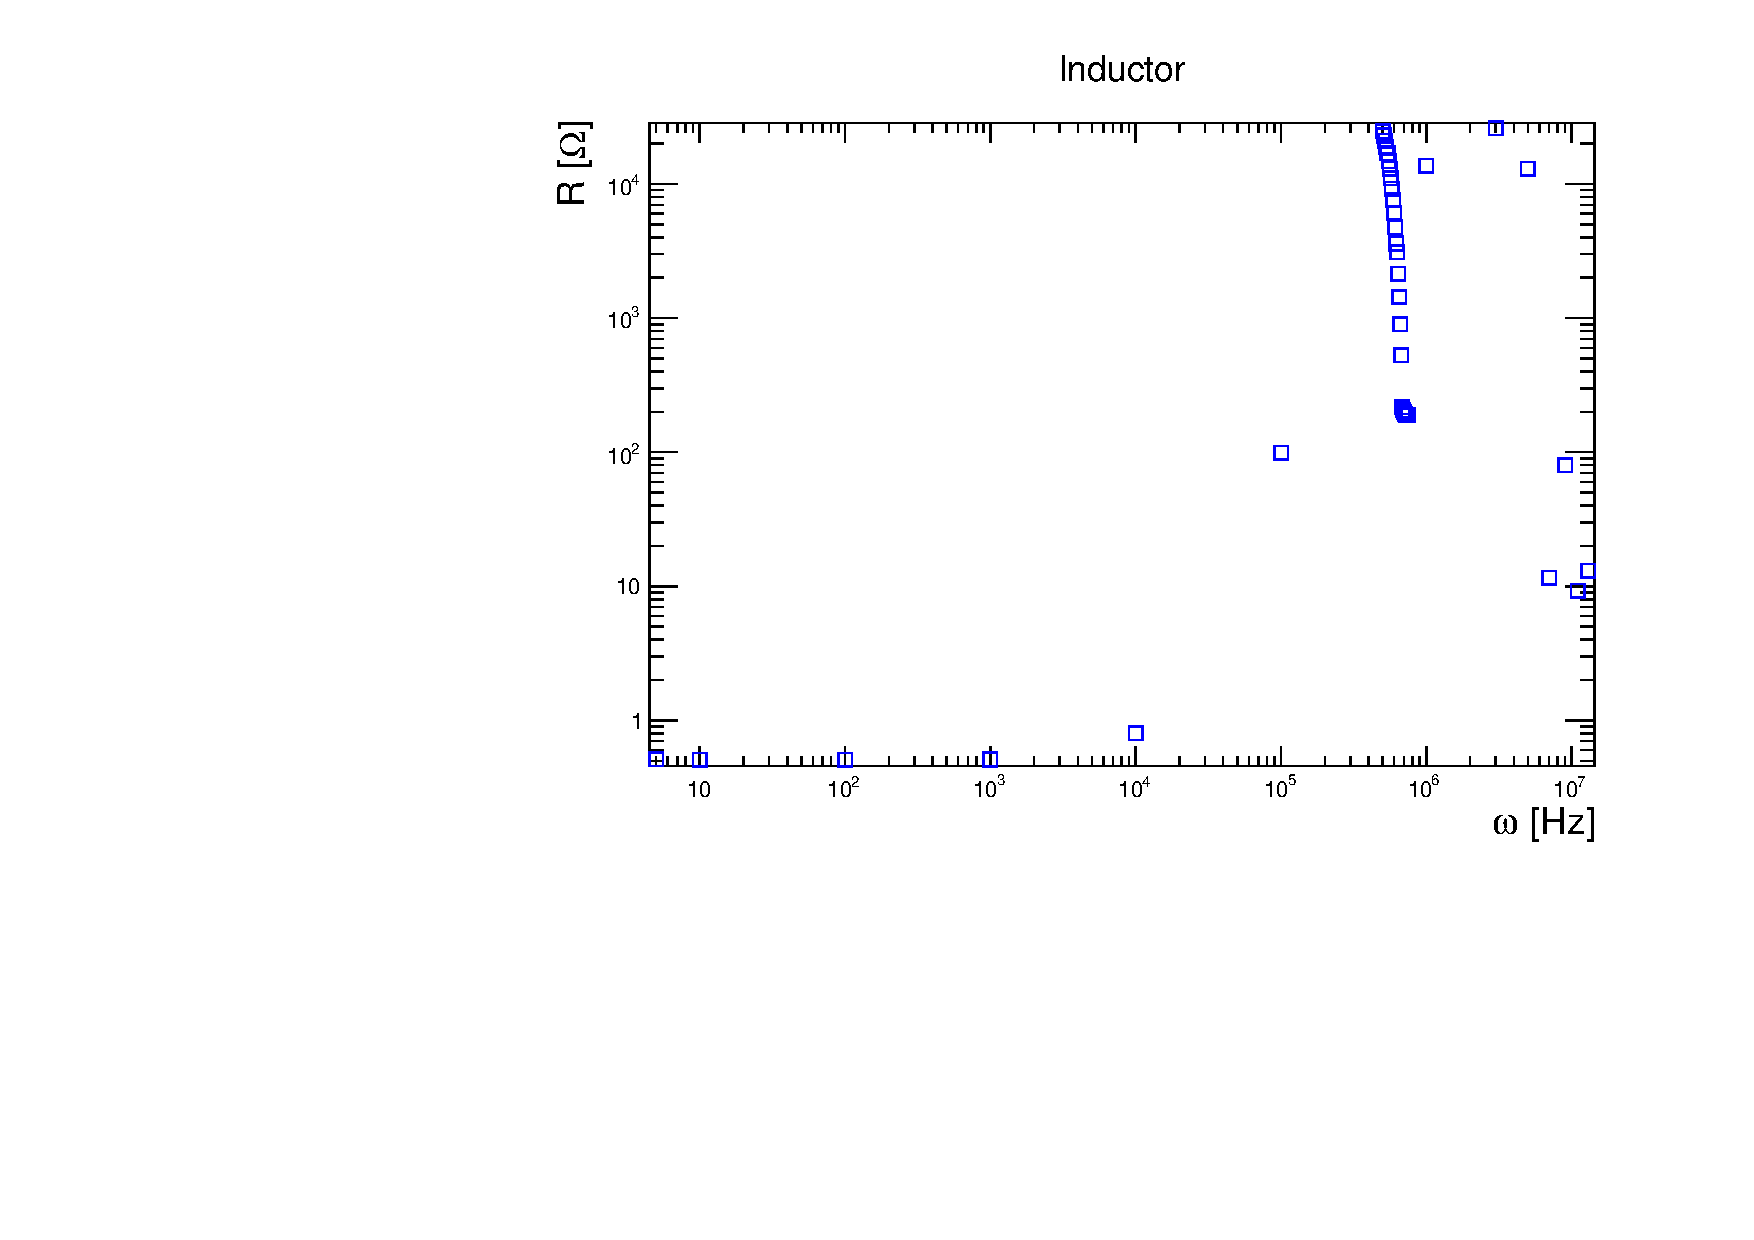
\includegraphics[width=1\linewidth]{pdf/c1_LR.pdf}} \\
    \end{minipage}
    \hfill
    \begin{minipage}[h]{0.47\linewidth}
        \center{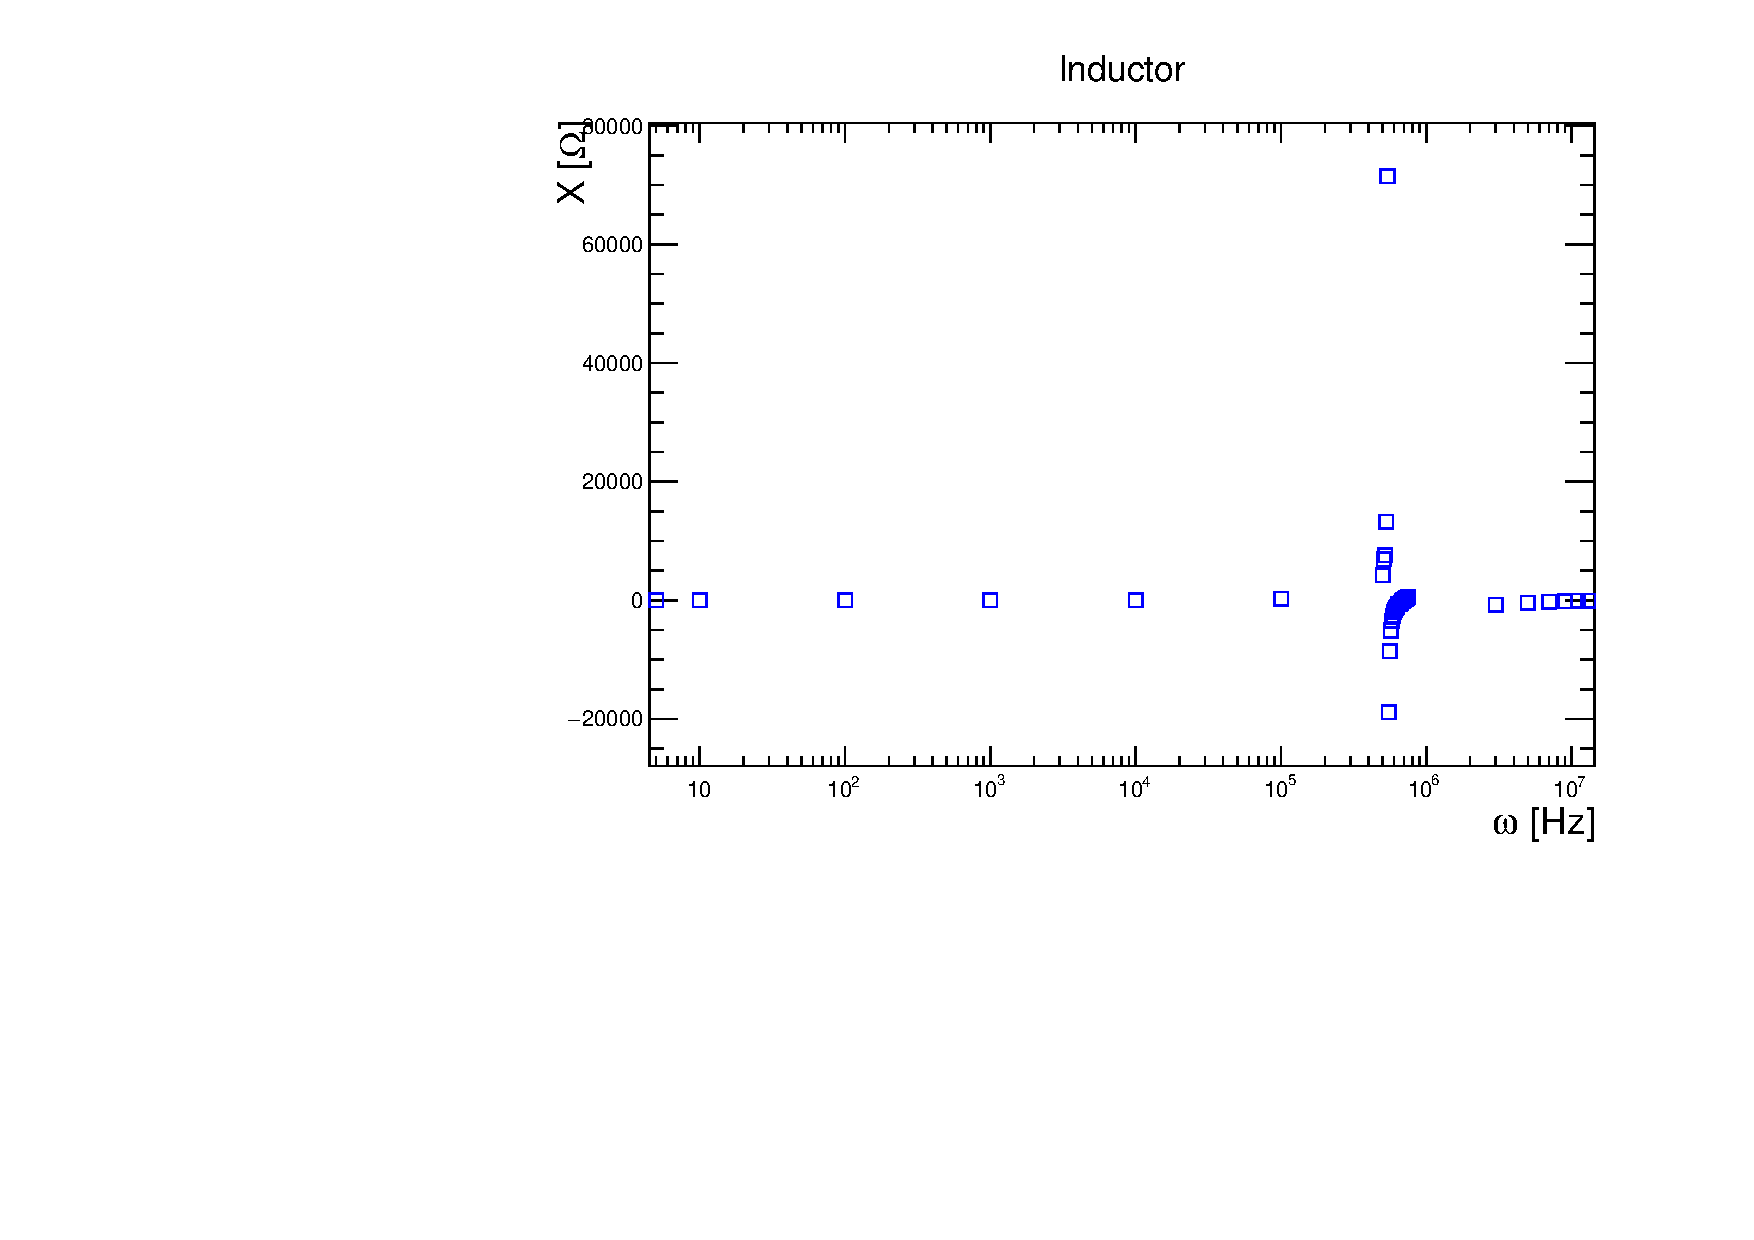
\includegraphics[width=1\linewidth]{pdf/c1_LX.pdf}}\\
    \end{minipage}
    \caption{Залежність активного та реактивного опору котушки від частоти}
    \label{fig:part23}
\end{figure}

Взагалі, робота з даним приладом варта 2 пострілам в голову, адже випадковим чином підібрані знаки, та інколи числа на його екрані не дають в спокійному режимі зняти потрібні покази.